\documentclass[11pt]{article}
\usepackage[margin=1in]{geometry}
\usepackage{booktabs}
\usepackage{graphicx}
\usepackage{xcolor}
\usepackage{abstract}
\usepackage{caption}
\usepackage{subcaption}
\usepackage{enumitem}
\usepackage{float}
\usepackage[numbers]{natbib}
\usepackage{amsmath}
\usepackage{placeins}
\usepackage{tabularx}
\usepackage{microtype}
\usepackage{needspace}
\usepackage{xurl}
\usepackage{etoolbox}
\usepackage{hyperref}
\hypersetup{colorlinks=true, linkcolor=blue, citecolor=blue, urlcolor=blue}
% Keep section heads with following material. Prefer needspace over a hard
% FloatBarrier here: flushing floats before every \section was leaving large
% empty regions (e.g. orphaned ``15'' before Forensic Case Studies).
\preto{\section}{\needspace{10\baselineskip}}
\preto{\subsection}{\needspace{4\baselineskip}}
\captionsetup{skip=3pt, font=small, justification=raggedright, singlelinecheck=false}
\setlength{\textfloatsep}{8pt plus 2pt minus 2pt}
\setlength{\floatsep}{8pt plus 2pt minus 2pt}
\setlength{\intextsep}{8pt plus 2pt minus 2pt}
\setlength{\abovecaptionskip}{4pt}
\setlength{\belowcaptionskip}{2pt}
\renewcommand{\topfraction}{0.92}
\renewcommand{\bottomfraction}{0.85}
\renewcommand{\textfraction}{0.08}
\renewcommand{\floatpagefraction}{0.85}
\setcounter{topnumber}{3}
\setcounter{bottomnumber}{2}
\setcounter{totalnumber}{5}
\clubpenalty=10000
\widowpenalty=10000
\displaywidowpenalty=10000
\brokenpenalty=10000
\emergencystretch=1.5em
\raggedbottom
\newcommand{\ttpath}[1]{\path{#1}}
\hyphenation{granularity quantisation quantization compressor compressors divergence}

\title{\textbf{When Does Compressed KV Start Lying?}\\[0.4em]
\large Token-Level Drift in KV Cache Compression}
\author{ExactKV Project}
\date{June 2026}

\begin{document}
\maketitle

\noindent\textbf{Key takeaways.}
ExactKV compares compressed-KV greedy decoding to full-precision greedy decoding.
\emph{Drift \%} $=$ share of prompts with $\geq$1 differing token.
\emph{First divergence} $=$ that token index.
(1)~matched hierarchy: \texttt{int4\_sim} Mistral \textbf{0\%, 23\%, 97\%}, Llama
\textbf{17\%, 26\%, 91\%} (code, tools, reading) at shared budgets.
(2)~BFCL length still scales 9\% to 62\%.
(3)~unguarded lossy can ship wrong fields. ExactKV recovers full-KV-valid outputs.
Details: Appendix~A,
\href{https://utkarshg20.github.io/ExactKV/}{project site},
\href{https://drive.google.com/file/d/1W2_dyc1QOBHTjc94yKPpQ-j7JKk04dln/view?usp=sharing}{PDF},
and the reproduction guide in the
\href{https://github.com/utkarshg20/ExactKV}{public repository}.

\begin{abstract}
Lossy KV-cache compression is widely deployed, but most evaluations report aggregate
quality and stop there. ExactKV is a compressor-agnostic \textbf{crash-test framework}
that measures first-divergence index, draft acceptance, unguarded lossy damage, and
\texttt{exactkv\_failure} under verifier-mediated semantics.

Across \textbf{8,132 GPU cells} on Llama-3.1-8B and Mistral-7B
(Appendix benchmark card)\footnote{Six built-in compressor classes: \texttt{noop},
\texttt{int8}, \texttt{int6\_sim}, \texttt{int4\_per\_vec\_sim}, \texttt{int4\_sim},
H2O-style eviction (\texttt{h2o\_sim}). External adapters evaluated separately
(Section~\ref{sec:faithful-compressors}). \texttt{exactkv\_failures=0} is a harness
invariant, not the scientific headline.}, four main findings (glance table below):

\begin{enumerate}
\item \textbf{Matched budgets:} Mistral 0\%, 23\%, 97\%, Llama 17\%, 26\%, 91\%
  (\texttt{int4\_sim}). H2O eviction 100\% on LongBench.
\item \textbf{Within-task length:} BFCL \texttt{int4\_sim} 9\% to 62\% (mnt 16 to 256).
\item \textbf{Three failure modes:} near-tie (int8), distribution shift (\texttt{int4\_sim}),
  attention destruction (H2O) over 1{,}103 divergent cells.
\item \textbf{Recovery:} BFCL validity \textbf{318/318} when full-KV valid; MBPP 12/12
  (Llama); LongBench overlap 100\% vs full-KV.
\end{enumerate}

\begin{sloppypar}
\noindent\texttt{int6\_sim} and \texttt{int4\_per\_vec\_sim} are GPU-validated
non-catastrophic on structured tasks (extended validation, 1{,}568 cells).
\textbf{Faithful upstream adapters} (1{,}568 appendix cells): TurboQuant is
task-conditional ($\sim$65\% LongBench); \texttt{int8} remains the only
non-catastrophic real compressor in that grid (8.3\% combined).
Drift is jointly governed by task, length, compressor class, and granularity.
Results are \textbf{not} benchmark scores, production claims, or a reproduction of
VeriCache~\citep{vericache2026}.
\end{sloppypar}
\end{abstract}

\section{Introduction}
Lossy KV-cache compression is widely deployed as a transparent optimization for
LLM inference. Under greedy decoding, a single perturbed logit can flip the
argmax, after which trajectories diverge. Aggregate metrics (perplexity,
LongBench, task accuracy) average over this divergence and hide \emph{where}
it begins, \emph{how severe} it is, and \emph{which compressor design choices}
drive it.

\begin{sloppypar}
ExactKV reframes KV-cache evaluation around a single diagnostic question:
\textbf{at what generated token does the compressed-cache path first stop
matching full-KV greedy decoding?} We answer this with a compressor-agnostic
crash-test framework that runs a draft/verify/commit loop and records
first-divergence index, draft acceptance, verifier agreement, and exactness
failures per cell.
\end{sloppypar}

\textbf{Contributions:}
\begin{enumerate}
\item A \textbf{compressor-agnostic crash-test framework} with leaderboard-style
  reporting for token-level drift, first divergence, acceptance, and exactness
  failures (\S3--5).
\item \textbf{Empirical map of when compressors drift}. matched task$\times$budget
  hierarchy, within-task length scaling, eviction vs quantization (glance table;
  Table~\ref{tab:matched-factorial}, \S6.12).
\item A \textbf{logit autopsy} over 1{,}103 divergent cells with three failure modes
  (\S\ref{sec:autopsy-main}, \S\ref{sec:forensic-cases}).
\item \textbf{Unguarded lossy damage vs verifier recovery} across three families;
  cost sketch \S9.1 (\S\ref{sec:downstream}).
\item \textbf{8,132 headline GPU cells} plus a 1{,}568-cell faithful-adapter appendix
  and GPU validation of \texttt{int6\_sim}/\texttt{int4\_per\_vec\_sim}
  (\S6, Sections~\ref{sec:int6}--\ref{sec:int4pervec}).
\end{enumerate}

\subsection{Shared problem framing with VeriCache}
VeriCache~\citep{vericache2026} and ExactKV share the observation that lossy KV
may look acceptable on short or aggregate metrics but \textbf{diverges more as
decoding continues}, and catastrophic for code and tool-calling. VeriCache uses
compressed KV to \textbf{draft} and full KV to \textbf{verify/correct}, guaranteeing
\textbf{identical greedy output} to full-KV inference.

\subsection{Where ExactKV diverges from VeriCache}
VeriCache is a \textbf{serving/system} paper. Its contribution is not merely
``draft then verify.'' It makes that loop practical by: (1)~keeping compressed KV
on GPU, (2)~keeping full KV in CPU/storage, loading only for verification,
(3)~\textbf{cross-resource staggering} (HBM-bound draft vs interconnect-bound
verify), (4)~reporting serving throughput (up to ${\sim}4\times$ vs full-KV in
their evaluation) with identical outputs.

ExactKV is an \textbf{evaluation crash-test}. It measures first divergence,
acceptance, and exactness failures, \emph{not} deployment throughput. It does
\emph{not} reproduce VeriCache scheduling or memory tiering.

\subsection{Main Findings at a Glance}

\begin{table}[htbp]
\centering\small
\begin{tabularx}{\textwidth}{@{}c>{\raggedright\arraybackslash}p{3.6cm}X@{}}
\toprule
\textbf{\#} & \textbf{Finding} & \textbf{Key number} \\
\midrule
1 & Matched task-family hierarchy (both models)
  & \texttt{int4\_sim}: Mistral 0\%, 23\%, 97\%; Llama 17\%, 26\%, 91\% \\
2 & Generation length (within-task control)
  & \texttt{int4\_sim} mnt=16: 9\% $\to$ mnt=256: 62\% ($7\times$) \\
3 & Eviction $>$ quantization
  & H2O-style 75\% kept $\to$ 100\% LongBench divergence \\
4 & Three distinct failure modes
  & int8 near-tie (rank 2.4, fdi=22); \texttt{int4\_sim} shift (rank 3.5, fdi=8);
    H2O destruction (rank 6.7, fdi=1) \\
5 & Unguarded lossy + recovery
  & BFCL 318/318; MBPP 12/12 (Llama); LongBench overlap 100\% (\S9.1) \\
6 & Compressor design curve
  & int8 $\to$ int6 $\to$ int4 per-vec $\to$ int4 sim $\to$ H2O
    (Table~\ref{tab:core-curve}) \\
7 & Faithful adapters reinforce hierarchy
  & TurboQuant $\sim$0--5\% code/tool, $\sim$65\% LongBench; int8 8.3\% combined \\
\bottomrule
\end{tabularx}
\caption{Main findings summary. Cross-family spans are observational; BFCL length is
the controlled within-task axis. \texttt{exactkv\_failures=0} is a harness invariant,
not the headline.}
\end{table}

\section{Definitions}
\subsection{Reference paths}
\begin{itemize}[noitemsep]
\item \textbf{Full-KV reference:} greedy generation with uncompressed KV.
\item \textbf{Lossy path:} compressed-KV greedy without verifier.
\item \textbf{ExactKV path:} verifier-mediated draft/verify/commit (\texttt{ExactKVGenerator}).
\end{itemize}

\subsection{Metrics (formal)}
\begin{table}[htbp]
\centering\small
\caption{Core metrics (formal definitions).}
\label{tab:metrics-formal}
\begin{tabularx}{\textwidth}{@{}>{\raggedright\arraybackslash}p{0.30\textwidth}>{\raggedright\arraybackslash}X@{}}
\toprule
\textbf{Metric} & \textbf{Definition} \\ \midrule
\texttt{first\_divergence\_index} &
  First position where the \emph{lossy} token $\neq$ full-KV greedy (before correction). \\
\texttt{acceptance\_rate} &
  \texttt{total\_accepted / total\_drafted} across verification rounds. \\
\texttt{exactkv\_failure} &
  Final ExactKV output $\neq$ full-KV greedy (verifier/commit failure). \\
\texttt{divergence\_rate} &
  Fraction of cells with lossy-path divergence. \\
\texttt{divergence\_stability} &
  $1 - \texttt{divergence\_rate}$ (complement). \\
\texttt{compression\_ratio} &
  Stored tensor byte ratio only (not active GPU memory). \\
\bottomrule
\end{tabularx}
\end{table}

\begin{sloppypar}
\textbf{Corrections vs rejections:} \texttt{total\_rejected} counts rejected
\emph{draft tokens}, \texttt{total\_corrections} counts verification \emph{rounds}
with a correction. For \texttt{int4\_sim}: 1284/1502 accepted, 218 rejected tokens,
\textbf{116 correction rounds}.
\end{sloppypar}

\subsection{Algorithm}
\begin{verbatim}
Prefill -> FullKVState + CompressedKVState
while generated < max_new_tokens:
  DRAFT from compressed KV (up to draft_len tokens)
  VERIFY each token vs full-KV greedy
  COMMIT accepted prefix, correct on mismatch
  ALIGN compressed state from authoritative full KV
return ExactKV output_ids
\end{verbatim}
Greedy decoding only in this release.

\section{Method}
Each \textbf{cell} is $(\text{model}, \text{compressor}, \text{prompt},
\texttt{max\_new\_tokens})$ with \texttt{draft\_len=4}, \texttt{seed=0}. Three
modes per cell: \textbf{full}, \textbf{lossy}, \textbf{exactkv}.

\noindent\textbf{Leaderboard-style score} (not an official benchmark ranking):
\[
\text{score} = 0.35\,a + 0.25\,v + 0.20\,\hat{d} + 0.10\,(1-f) + 0.10\,s
\]
\begin{center}
\small
\begin{tabular}{cl}
\toprule
\textbf{Symbol} & \textbf{Meaning} \\
\midrule
$a$ & Mean draft acceptance rate (\texttt{total\_accepted}/\texttt{total\_drafted}) \\
$v$ & Mean verifier agreement ($=a$ on the scale panel in this release) \\
$\hat{d}$ & Normalized first-divergence index $\in[0,1]$: mean FDI$/\texttt{max\_new\_tokens}$, or 1.0 if none \\
 & (later / no divergence is better) \\
$f$ & ExactKV failure rate (ExactKV output $\neq$ full-KV) \\
$s$ & Stability subscore (Exp-116 when available; else $1-$ divergence rate) \\
\bottomrule
\end{tabular}
\end{center}

\section{Experimental Setup}
\begin{table}[htbp]
\centering\small
\caption{Headline release panel (1,500 cells; Appendix inventory).}
\label{tab:experimental-setup}
\begin{tabularx}{\textwidth}{@{}>{\raggedright\arraybackslash}p{0.28\textwidth}>{\raggedright\arraybackslash}X@{}}
\toprule
\textbf{Parameter} & \textbf{Value} \\ \midrule
Panel ID & \texttt{phase\_a\_unified\_panel} \\
Total cells & \textbf{1500} = $2 \times 5 \times 50 \times 3$ \\
Models & Llama-3.1-8B (750), Mistral-7B (750) \\
Stack & torch 2.8.0+cu128, transformers 5.12.1, ExactKV (this report) \\
\texttt{draft\_len} & 4 \quad \texttt{max\_new\_tokens} $\in \{4,8,16\}$ \\
Decoding & Greedy only \\
Prompts & 50 variants from 4 stress templates (capital, math, JSON, code) \\
Categories & capital\_france 390, simple\_math 390, json\_tool 360, code\_fn 360 \\
Execution & Sequential per model, \texttt{deterministic\_mode=false} \\
\bottomrule
\end{tabularx}
\end{table}

\textbf{Validated compressors:} \texttt{noop}, \texttt{int8}, \texttt{int4\_sim}.
Real KIVI/KVQuant/SnapKV/TurboQuant are not in the headline panel.
Unvalidated proxy slots in raw artifacts are excluded from analysis
(Limitations~\S\ref{sec:limitations}).

\begin{sloppypar}
\textbf{1,560 GPU cells} total: 216 Llama-3.1-8B cells across bundled
LongBench/RULER/BFCL/HumanEval pilots; 144 MBPP cells across both models;
1,200 BFCL export-50 tool-call drift cells across both models;
\texttt{exactkv\_failures=0} throughout. Not official benchmark scores.
\end{sloppypar}

\section{Results: Validated Compressors}
Table~\ref{tab:validated-compressors}: built-in compressors with direct ExactKV
integration (\texttt{noop}, \texttt{int8}, \texttt{int4\_sim}). Aggregates from
the headline release panel (300 cells each: 150 per model).

\begin{figure}[htbp]
\centering
\begin{subfigure}{0.48\textwidth}
  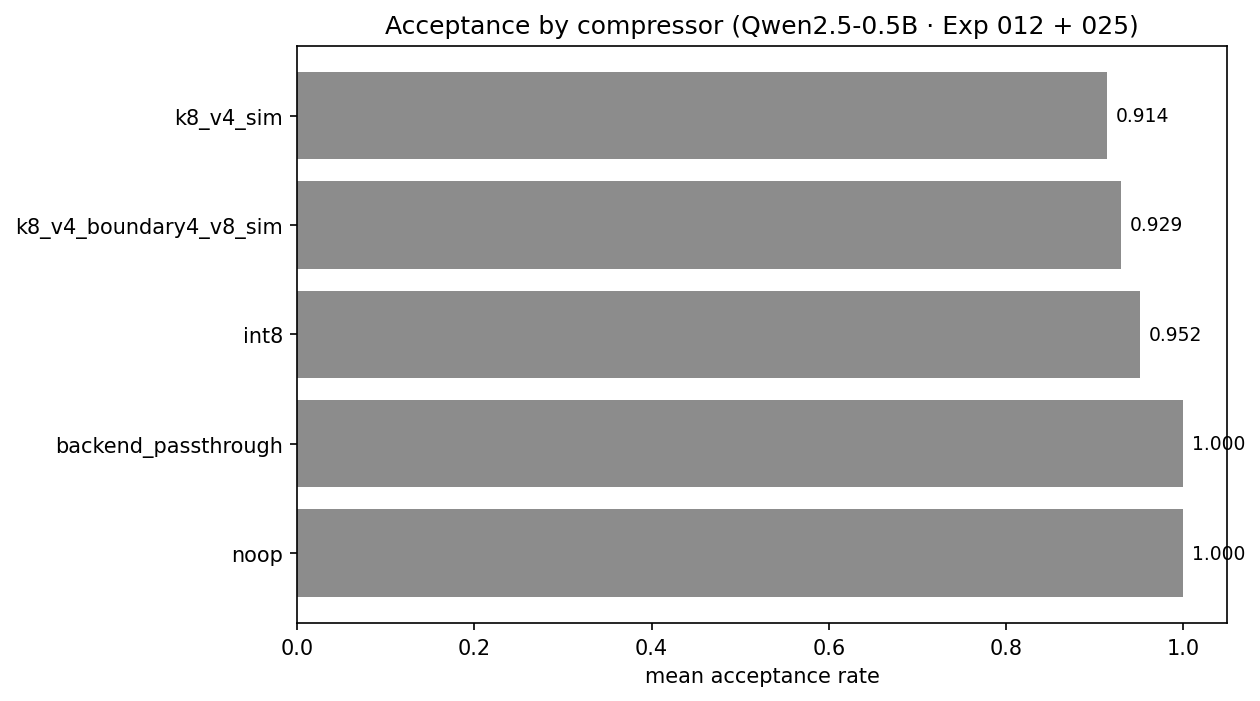
\includegraphics[width=\linewidth]{figures/acceptance_by_compressor.png}
  \caption{Acceptance by compressor.}
\end{subfigure}\hfill
\begin{subfigure}{0.48\textwidth}
  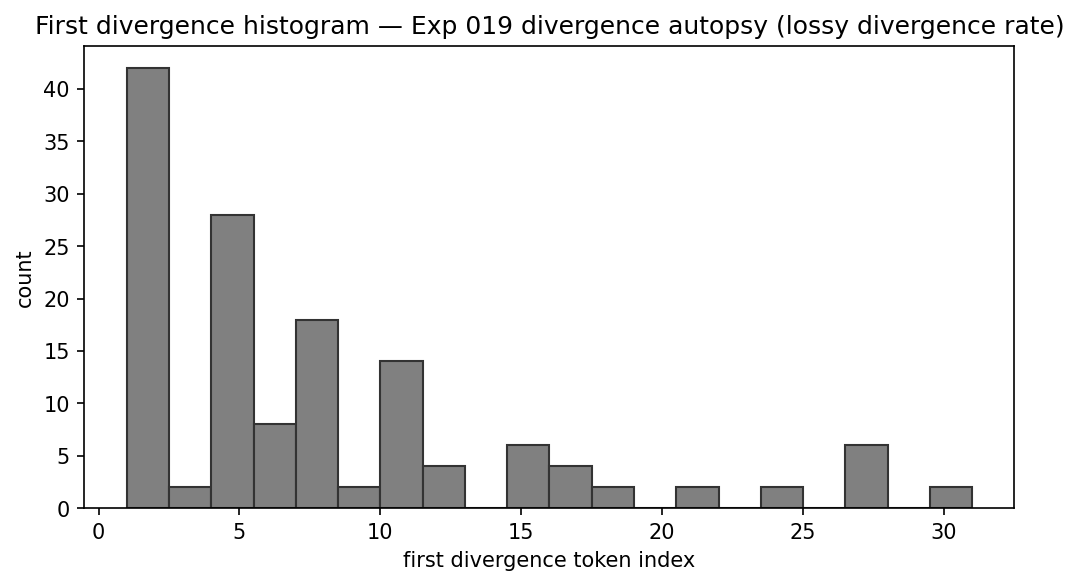
\includegraphics[width=\linewidth]{figures/first_divergence_histogram.png}
  \caption{First-divergence distribution.}
\end{subfigure}
\caption{Release benchmark visuals from the headline panel.}
\end{figure}

\begin{table}[htbp]
\centering\small
\renewcommand{\arraystretch}{1.12}
\setlength{\tabcolsep}{5pt}
\begin{tabular}{@{}lrrrrrr@{}}
\toprule
\textbf{Compressor} & \textbf{Cells} & \textbf{Accept.} & \textbf{Div.$^\dagger$} & \textbf{Stab.} & \textbf{FDI$^\S$} & \textbf{Fail.} \\ \midrule
\texttt{noop} & 300 & 1.000 & 0.00 & 1.00 & n/a & 0.00 \\
\texttt{int8} & 300 & 1.000 & 0.00 & 1.00 & n/a & 0.00 \\
\texttt{int4\_sim} & 300 & 0.851 & 0.52 & 0.48 & 2.0 & 0.00 \\
\bottomrule
\end{tabular}
\caption{Built-in compressors from the headline panel.
  $^\dagger$Lossy-path divergence fraction.
  $^\S$Mean first-divergence index over divergent cells only.
  Histogram for \texttt{int4\_sim}: index 1$\to$78, 3$\to$39, 5$\to$24, 8$\to$13 cells.}
\label{tab:validated-compressors}
\end{table}

\texttt{int8}/\texttt{noop}: no lossy divergence. \texttt{int4\_sim}: drifts in
52\% of cells yet \texttt{exactkv\_failure=0} because the verifier corrects.

\textbf{Leaderboard-style scores} (formula above; Appendix inventory):

\begin{table}[htbp]
\centering\small
\begin{tabular}{l l r r r r r}
\toprule
\textbf{Compressor} & \textbf{Model} & \textbf{Score} & \textbf{Accept.} & \textbf{Div. rate$^\dagger$} & \textbf{Stab.} & \textbf{Cells} \\ \midrule
\texttt{noop} & Llama-3.1-8B & 1.000 & 1.000 & 0.000 & 1.000 & 150 \\
\texttt{int8} & Llama-3.1-8B & 1.000 & 1.000 & 0.000 & 1.000 & 150 \\
\texttt{noop} & Mistral-7B & 1.000 & 1.000 & 0.000 & 1.000 & 150 \\
\texttt{int8} & Mistral-7B & 0.983 & 1.000 & 0.000 & 0.827 & 150 \\
\texttt{int4\_sim} & Llama-3.1-8B & 0.859 & 0.852 & 0.520 & 0.480 & 150 \\
\texttt{int4\_sim} & Mistral-7B & 0.851 & 0.837 & 0.507 & 0.493 & 150 \\
\bottomrule
\end{tabular}
\caption{Leaderboard-style scores for validated built-in compressors.
$^\dagger$Div.\ rate = raw lossy-path token divergence fraction (same metric as Table~\ref{tab:validated-compressors}).
\texttt{int8} Mistral: divergence\_rate=0.000 (zero cells diverge). \texttt{Stab.}=0.827
is the \textbf{leaderboard stability subscore}, which
is distinct from the formal metric $\text{divergence\_stability} = 1 - \text{divergence\_rate}$
(Table~\ref{tab:metrics-formal}). Under the formal metric, \texttt{int8} Mistral
divergence\_stability=1.000.}
\label{tab:leaderboard-scores}
\end{table}

\subsection{Metric interpretation}
\begin{sloppypar}
Divergence rate and acceptance rate measure \emph{different} failure modes. Low
lossy-path divergence does not imply high verifier acceptance (and vice versa).
Example: \texttt{int4\_sim} at \texttt{max\_new\_tokens=16} can show first
divergence at index 8 with acceptance 0.94, how late drift occurs matters.
\end{sloppypar}
\subsection{Evidence-plus long-context panel}
\textbf{Source:} evidence-plus panel (RunPod A5000, June 2026; Appendix inventory).
144 cells = $2 \times 6 \times 2 \times 3 \times 2$, prefill buckets 512/1024,
\texttt{max\_new\_tokens} $\in \{16,32\}$, built-in compressors only.
\begin{table}[htbp]
\centering\small
\begin{tabular}{lrrrr}
\toprule
Compressor & Cells & Accept. & Div.\ rate & Fail. \\ \midrule
\texttt{noop} & 48 & 1.000 & 0.00 & 0.00 \\
\texttt{int8} & 48 & 1.000 & 0.00 & 0.00 \\
\texttt{int4\_sim} & 48 & 0.985 & 0.31 & 0.00 \\
\bottomrule
\end{tabular}
\caption{Evidence-plus aggregates. \texttt{int4\_sim}: Mistral 41.7\%, Llama 20.8\% divergence (24 cells each).}
\end{table}
By context bucket (all compressors): 512$\to$11.1\% divergence, 1024$\to$9.7\%.
Diagnostic timing: mean 3854\,ms, p90 5178\,ms per cell (not serving throughput).

\subsection{External benchmark smoke panels}
{\sloppy\noindent\textbf{Source:} Llama-only external smoke (216 cells) and MBPP smoke
(144 cells). \texttt{exactkv\_failures=0} on all panels. 216-cell subset:
\texttt{noop}/\texttt{int8}: 0\%. 15 divergent cells (\texttt{int4\_sim} only).\par}

\begin{table}[htbp]
\centering\scriptsize
\setlength{\tabcolsep}{3.5pt}
\renewcommand{\arraystretch}{1.05}
\begin{tabular}{@{}llllrrrrrr@{}}
\toprule
\textbf{Panel} & \textbf{Src} & \textbf{Model} & \textbf{Ctx} & \textbf{MNT} & \textbf{n} & \textbf{Div.} & \textbf{Acc.} & \textbf{Fail} & \textbf{P90} \\ \midrule
LongBench & pilot & Llama & 2,4 & 16,32 & 72 & 0.083 & 0.994 & 0 & 8781 \\
RULER 2K--4K & pilot & Llama & 2,4 & 16,32 & 48 & 0.083 & 0.993 & 0 & 8793 \\
RULER 8K & pilot & Llama & 8 & 16,32 & 24 & 0.083 & 0.993 & 0 & 13640 \\
BFCL & pilot & Llama & 1,2 & 16,32 & 48 & 0.063 & 0.999 & 0 & 6342 \\
HumanEval & pilot & Llama & 1,2 & 32 & 24 & 0.000 & 1.000 & 0 & 6392 \\
\bottomrule
\end{tabular}
\caption{Llama-3.1-8B external smoke panels (216 cells, \texttt{noop}/\texttt{int8}/\texttt{int4\_sim}).
Drift metrics; not official scores. P90 is wall-clock ms.}
\label{tab:external-smoke}
\end{table}

\begin{table}[htbp]
\centering\scriptsize
\setlength{\tabcolsep}{3.5pt}
\renewcommand{\arraystretch}{1.05}
\begin{tabular}{@{}llllrrrrrr@{}}
\toprule
\textbf{Panel} & \textbf{Src} & \textbf{Models} & \textbf{Ctx} & \textbf{MNT} & \textbf{n} & \textbf{Div.} & \textbf{Acc.} & \textbf{Fail} & \textbf{P90} \\ \midrule
MBPP & pilot & Both & 0.5,1 & 16,32 & 144 & 0.021 & 0.999 & 0 & 5121 \\
\bottomrule
\end{tabular}
\caption{MBPP code-drift smoke (144 cells, \texttt{noop}/\texttt{int8}/\texttt{int4\_sim}).
Not pass@1; no test execution.}
\label{tab:external-mbpp}
\end{table}

\begin{table}[htbp]
\centering\scriptsize
\renewcommand{\arraystretch}{1.05}
\begin{tabular}{llrrrr}
\toprule
\textbf{Compressor} & \textbf{Model} & \textbf{Cells} & \textbf{Div.\ rate} & \textbf{CI\textsubscript{95} low} & \textbf{CI\textsubscript{95} high} \\ \midrule
\texttt{noop} & Llama-3.1-8B & 200 & 0.000 & 0.000 & 0.019 \\
\texttt{noop} & Mistral-7B & 200 & 0.000 & 0.000 & 0.019 \\
\texttt{int8} & Llama-3.1-8B & 200 & 0.000 & 0.000 & 0.019 \\
\texttt{int8} & Mistral-7B & 200 & 0.000 & 0.000 & 0.019 \\
\texttt{int4\_sim} & Llama-3.1-8B & 200 & 0.055 & 0.031 & 0.096 \\
\texttt{int4\_sim} & Mistral-7B & 200 & 0.170 & 0.124 & 0.228 \\
\bottomrule
\end{tabular}
\caption{BFCL export-50 tool-call drift panel (1,200 cells, both models, 50 prompts).
\texttt{exactkv\_failures=0}. Source: \texttt{bfcl\_export\_50\_raw.json}.
Drift measurement only (not JSON-completeness). \texttt{max\_new\_tokens}$\in\{16,32\}$.
Mistral-7B \texttt{int4\_sim} divergence (17.0\%) is $3\times$ Llama-3.1-8B (5.5\%).}
\label{tab:bfcl-export50}
\end{table}

Notable: LongBench \texttt{int4\_sim} 25\%. RULER 8192 \texttt{niah\_single} 33\%. BFCL pilot \texttt{int4\_sim} 18.75\%. BFCL export-50 \texttt{int4\_sim} 11.3\%
(Llama 5.5\%, Mistral 17.0\%). HumanEval zero drift. MBPP 3/144 divergent.
\texttt{int8}/\texttt{noop}: 0\% divergence on all panels.

\begin{table}[htbp]
\centering\small
\renewcommand{\arraystretch}{1.05}
\begin{tabular}{lrrrrr}
\toprule
\textbf{Panel} & \textbf{n} & \textbf{Div.} & \textbf{Rate} & \textbf{CI\textsubscript{95} low} & \textbf{CI\textsubscript{95} high} \\ \midrule
LongBench pilot & 72 & 6 & 8.3\% & 3.9\% & 17.0\% \\
RULER 2K--4K & 48 & 4 & 8.3\% & 3.3\% & 19.7\% \\
RULER 8K & 24 & 2 & 8.3\% & 2.3\% & 25.8\% \\
BFCL pilot & 48 & 3 & 6.3\% & 2.2\% & 16.8\% \\
HumanEval pilot & 24 & 0 & 0.0\% & 0.0\% & 14.2\% \\
MBPP pilot & 144 & 3 & 2.1\% & 0.7\% & 6.0\% \\
BFCL exp-50 \texttt{int4\_sim} Llama & 200 & 11 & 5.5\% & 3.1\% & 9.6\% \\
BFCL exp-50 \texttt{int4\_sim} Mistral & 200 & 34 & 17.0\% & 12.4\% & 22.8\% \\
BFCL exp-50 \texttt{int8}/\texttt{noop} & 800 & 0 & 0.0\% & 0.0\% & 0.5\% \\
\midrule
All 216 ext.\ cells & 216 & 15 & 6.9\% & 4.3\% & 11.1\% \\
\bottomrule
\end{tabular}
\caption{Wilson 95\% CIs on divergence rate (panel-level).
``All 216 ext.\ cells'' refers to the \textbf{initial} LongBench/RULER/BFCL/HumanEval pilot panel (first workflow, Llama-only). The full 1,560-cell external smoke total includes MBPP and BFCL export-50.}
\label{tab:ci-divergence}
\end{table}

\textbf{Overall acceptance (initial 216 ext.\ pilot cells):} Full-acceptance rate 93.7\%, Wilson 95\% CI [90.5\%, 96.8\%].
Source: \texttt{analysis\_pack.json} $\to$ \texttt{totals.acceptance\_full\_rate\_ci95}.

\subsection{KIVI offline compressor panel, real HF results (640 cells)}
\textbf{Source:} \texttt{kivi\_longbench\_hf\_raw.json} (320 cells) + \texttt{kivi\_mbpp\_hf\_raw.json} (320 cells).
RunPod RTX A5000, June 2026. \texttt{exactkv\_failures=0} on all 640 cells.

\begin{table}[htbp]
\centering\small
\renewcommand{\arraystretch}{1.05}
\begin{tabular}{lrrrrrr}
\toprule
\textbf{Compressor} & \textbf{LB div.} & \textbf{LB acc.} & \textbf{MBPP div.} & \textbf{MBPP acc.} & \textbf{Fail.} \\ \midrule
\texttt{noop} & 0.0\% & 1.000 & 0.0\% & 1.000 & 0 \\
\texttt{int8} & 13.8\% & 0.994 & 0.0\% & 1.000 & 0 \\
\texttt{int4\_sim} & 91.2\% & 0.818 & 5.0\% & 0.995 & 0 \\
\texttt{kivi\_offline} & \textbf{100.0\%} & \textbf{0.004} & \textbf{100.0\%} & \textbf{0.001} & \textbf{0} \\
\bottomrule
\end{tabular}
\caption{KIVI offline compressor panel (80 cells each × 4 compressors × 2 datasets).
\texttt{kivi\_offline} produced catastrophic \textbf{adapter-level} drift in this
ExactKV integration (near-zero acceptance). Because this is an offline simulate-path
adapter rather than KIVI production CUDA/Triton serving, these results diagnose the
adapter/integration path, \emph{not} the KIVI algorithm as deployed.
ExactKV detected and corrected all cells (\texttt{exactkv\_failures=0}).
Real HF \texttt{int4\_sim} drift (LB: 91.2\%) greatly exceeds bundled pilot (20.8\%).}
\label{tab:kivi-panel}
\end{table}

\section{ExactKV-HF-LongBench Drift Panel (v2.6, Complete)}

\textbf{Status:} Complete. 720 cells, both models, \texttt{exactkv\_failures=0}.

\begin{table}[htbp]
\centering\small\setlength\tabcolsep{5pt}
\renewcommand{\arraystretch}{1.05}
\begin{tabular}{llrrrrrl}
\toprule
\textbf{Model} & \textbf{Compressor} & \textbf{n} & \textbf{Div.} & \textbf{Rate} & \textbf{CI$_{95}$} & \textbf{Mean acc.} & \textbf{EKV fail} \\
\midrule
Llama-3.1-8B & noop      & 120 &   0 &  0.0\% & [0.0\%,\,3.1\%] & 1.000 & 0 \\
Llama-3.1-8B & int8      & 120 &  33 & 27.5\% & [20.3\%,\,36.1\%] & 0.988 & 0 \\
Llama-3.1-8B & int4\_sim  & 120 & 110 & \textbf{91.7\%} & [85.3\%,\,95.4\%] & 0.825 & 0 \\
\midrule
Mistral-7B   & noop      & 120 &   0 &  0.0\% & [0.0\%,\,3.1\%] & 1.000 & 0 \\
Mistral-7B   & int8      & 120 &  26 & 21.7\% & [15.2\%,\,29.9\%] & 0.988 & 0 \\
Mistral-7B   & int4\_sim  & 120 & 107 & \textbf{89.2\%} & [82.3\%,\,93.6\%] & 0.861 & 0 \\
\midrule
All (int4\_sim) & all & \textbf{240} & \textbf{217} & \textbf{90.4\%} & \textbf{[86.1\%,\,93.5\%]} & 0.843 & \textbf{0} \\
\bottomrule
\end{tabular}
\caption{ExactKV-HF-LongBench v2.6 (720 cells, 10 real HF subsets, contexts 2K/4K/8K,
\texttt{mnt}=32/64, both models). int4\_sim: \textbf{90.4\%} divergence on long-context
open-text tasks, highest across all ExactKV panels. int8 shows 24.6\%, unlike its 0\%
on BFCL/MBPP/RULER. \texttt{exactkv\_failures=0}. Median first-div index: 4 (Llama) / 6 (Mistral).}
\label{tab:hf-longbench-v26}
\end{table}

\textbf{Key finding (task-type sensitivity):}
Real HF LongBench open-text reading/summarization at 2K--8K prefill produces
\textbf{very high int4\_sim divergence} (90.4\%), the highest seen across all ExactKV panels.
Even int8 shows 24.6\% divergence on LongBench tasks, unlike its 0\% on BFCL, MBPP, and
RULER. Divergence occurs very early (median token 4--6 out of 32--64 generated).
\texttt{exactkv\_failures=0} across all 720 cells.

Table~\ref{tab:longbench-subset} shows per-subset int4\_sim divergence.
\texttt{lcc} (code completion) is notably lower for Mistral (42\%), consistent with
code tasks being more stable under int4\_sim across panels.

\begin{table}[htbp]
\centering\small\setlength\tabcolsep{4pt}
\renewcommand{\arraystretch}{1.05}
\begin{tabular}{lllrr}
\toprule
\textbf{Subset} & \textbf{Type} & & \textbf{Llama int4\_sim} & \textbf{Mistral int4\_sim} \\
\midrule
2wikimqa & multi-hop QA & & 12/12 (100\%) & 12/12 (100\%) \\
gov\_report & summarization & & 11/12 (92\%) & 12/12 (100\%) \\
hotpotqa & multi-hop QA & & 12/12 (100\%) & 12/12 (100\%) \\
\textbf{lcc} & \textbf{code completion} & & \textbf{11/12 (92\%)} & \textbf{5/12 (42\%)} \\
multifieldqa\_en & multi-field QA & & 6/12 (50\%) & 10/12 (83\%) \\
narrativeqa & reading comp. & & 12/12 (100\%) & 12/12 (100\%) \\
passage\_retr. & doc.\ retrieval & & 12/12 (100\%) & 12/12 (100\%) \\
qasper & academic QA & & 12/12 (100\%) & 12/12 (100\%) \\
samsum & dialogue summ. & & 10/12 (83\%) & 12/12 (100\%) \\
trec & classification & & 12/12 (100\%) & 8/12 (67\%) \\
\bottomrule
\end{tabular}
\caption{Per-subset int4\_sim divergence in HF LongBench v2.6 (2K/4K/8K context,
\texttt{mnt}=32/64). \texttt{lcc} (code completion) shows lower divergence for Mistral
(42\%) vs.\ reading-comprehension tasks (100\%), consistent with code-task stability
across all ExactKV panels. \texttt{exactkv\_failures=0} for all 720 cells.}
\label{tab:longbench-subset}
\end{table}

\section{BFCL Tool-Call Validity Panel (v2.7, Complete, 1,200 cells)}

The 48-cell BFCL pilot used \texttt{max\_new\_tokens $\in$ \{16,\,32\}}, too short for
complete JSON tool calls. A dedicated 1,200-cell validity panel
(\texttt{max\_new\_tokens=128/256}) was completed with both models.

\begin{table}[htbp]
\centering\small\setlength\tabcolsep{5pt}
\renewcommand{\arraystretch}{1.05}
\begin{tabular}{llrrrr}
\toprule
\textbf{Compressor} & \textbf{Model} & \textbf{n} & \textbf{Div.} & \textbf{Rate} & \textbf{EKV fail} \\
\midrule
noop      & Llama   & 200 &   0 &  0.0\% & 0 \\
noop      & Mistral & 200 &   0 &  0.0\% & 0 \\
int8      & Llama   & 200 &   0 &  0.0\% & 0 \\
int8      & Mistral & 200 &   3 &  1.5\% & 0 \\
int4\_sim & Llama   & 200 &  90 & \textbf{45.0\%} & 0 \\
int4\_sim & Mistral & 200 & 111 & \textbf{55.5\%} & 0 \\
\midrule
\textbf{All (1,200)} & both & 1,200 & 204 & \textbf{17.0\%} & \textbf{0} \\
\bottomrule
\end{tabular}
\caption{BFCL tool-call validity panel v2.7 (1,200 cells, mnt=128/256, both models).
\texttt{int4\_sim} diverges 45.0\% on Llama and 55.5\% on Mistral with long generation,
vs 11\% at mnt=16/32, confirming generation length as a primary driver.
\texttt{int8} is near-zero. \texttt{exactkv\_failures=0} throughout.
Artifact: \texttt{bfcl\_validity\_v27\_merged\_raw.json}.}
\label{tab:bfcl-validity}
\end{table}

\section{H2O-Style Token-Eviction Panel (v2.8, Complete, 800 cells)}
\label{sec:h2o-panel}

\textbf{Status:} Complete. 800 cells, 5 eviction variants, both models,
\texttt{exactkv\_failures=0}. Artifact: \texttt{h2o\_v28\_merged\_raw.json}.

\textbf{Eviction mechanism:} \texttt{h2o\_sim\_75}, \texttt{h2o\_sim}, and
\texttt{h2o\_sim\_25} keep approximately 75\%, 50\%, and 25\% of prefill tokens
using a simplified heavy-hitter-style eviction heuristic (cumulative attention score
across heads). Lowest-scoring tokens are evicted after the full prefill. retained
tokens include attention sinks (positions 0--3) plus the highest-attention tokens
by recency/score. This approximates the H2O~\citep{zhang2023h2o} eviction policy
but omits the original online streaming update and GPU-efficient sparse-attention
kernel. Results characterize the eviction compressor \emph{class}, not the published
H2O system.

\textbf{Key result:} Even mild eviction (75\% of tokens kept) causes \textbf{100\%
divergence} on LongBench reading tasks for both models. The H2O-style simulation
reaches mean lossy rank 6.5--6.7 at divergence (vs.\ rank 3.5 for \texttt{int4\_sim}),
confirming attention destruction as a qualitatively distinct failure mode.
\texttt{exactkv\_failures=0} across all 800 cells.

\section{Cross-Panel Divergence Analysis: Task-Type Sensitivity}

Table~\ref{tab:cross-panel} summarises int4\_sim, int8, and noop divergence rates
across completed ExactKV panels. Cross-family rates are \textbf{observational}.

\noindent\textbf{Threat / confound.} Cross-family comparisons (MBPP vs BFCL vs LongBench)
change prompts, context buckets, and \texttt{max\_new\_tokens} together. The memorable
\texttt{int4\_sim} span 6\%$\to$90\% is \emph{not} a pure causal claim that task type alone
drives drift. Controlled axes: BFCL mnt 16 to 256 (fixed tool-call family) and LongBench
2K/4K/8K (fixed reading family). A matched task$\times$context$\times$\texttt{max\_new}
factorial with shared budgets confirms the hierarchy on both models
(Table~\ref{tab:matched-factorial}); prompts still differ by family.

\begin{table}[htbp]
\centering\small\setlength\tabcolsep{4pt}
\renewcommand{\arraystretch}{1.05}
\begin{tabular}{lllllrrr}
\toprule
\textbf{Panel} & \textbf{Task} & \textbf{Ctx} & \textbf{mnt} & \textbf{Models} & \textbf{noop} & \textbf{int8} & \textbf{int4\_sim} \\
\midrule
Headline (v1) & mixed & $\sim$500 & 16/32 & L+M & 0.0\% & 0.0\% & \textbf{51.3\%} \\
Evidence-plus (v2) & mixed & 512/1024 & 16 & L+M & 0.0\% & 0.0\% & \textbf{31.2\%} \\
MBPP code-drift & code & 512/1024 & 16/32 & L+M & 0.0\% & 0.0\% & \textbf{6.2\%} \\
BFCL export-50 & tool-call & 1K--2K & 16/32 & L+M & 0.0\% & 0.0\% & \textbf{11.2\%} \\
BFCL validity v2.7 & tool-call & 1K--2K & 128/256 & L+M & 0.0\% & 0.8\% & \textbf{50.3\%} \\
HF LongBench v2.6 & reading/summ. & 2K--8K & 32/64 & L+M & 0.0\% & 24.6\% & \textbf{90.4\%} \\
\bottomrule
\end{tabular}
\caption{Cross-panel int4\_sim/int8/noop divergence rates (observational across families).
noop=0\% throughout. Memorable span: code 6\% $<$ tool short 11\% $<$ tool long 50\% $<$
reading 90\%. confounded with context/\texttt{max\_new}. Within-task BFCL length
11\%$\to$50\% as mnt 16 to 256. Harness invariant \texttt{exactkv\_failures=0}.
L=Llama-3.1-8B, M=Mistral-7B.}
\label{tab:cross-panel}
\end{table}

\section{Mechanistic Analysis: Divergence Autopsy}
\label{sec:autopsy-main}

\begin{sloppypar}
The cross-panel observational hierarchy is supported by a token-level mechanistic analysis.
ExactKV stored top-5 full-KV and lossy logit distributions at each divergence point
(\texttt{--store-top-k-logits}), enabling a logit autopsy across 1{,}103 divergent cells
from v2.6, v2.7, and v2.8 panels.
\end{sloppypar}
\begin{table}[htbp]
\centering\small\setlength\tabcolsep{5pt}
\begin{tabular}{lrrrrrr}
\toprule
\textbf{Compressor} & \textbf{n div} & \textbf{top-1 flip} & \textbf{near-tie} & \textbf{mean margin} & \textbf{mean rank} & \textbf{med.\ fdi} \\
\midrule
int8 & 62 & 69\% & \textbf{66\%} & 0.116 & 2.4 & 22 \\
int4\_sim & 563 & 83\% & 26\% & 0.305 & 3.5 & 8 \\
h2o\_sim\_75 & 160 & \textbf{100\%} & 0\% & 0.545 & 6.5 & 1 \\
h2o\_sim & 160 & \textbf{100\%} & 0\% & 0.536 & 6.7 & 1 \\
h2o\_sim\_25 & 158 & \textbf{100\%} & 1\% & 0.551 & 6.5 & 1 \\
\bottomrule
\end{tabular}
\caption{Logit autopsy across 1,103 divergent cells. near-tie: full-KV margin $<0.05$.
fdi = first-divergence index. Three distinct failure modes: (1)~\emph{near-tie noise}
(int8), (2)~\emph{distribution shift} (int4\_sim), (3)~\emph{attention destruction}
(H2O-style). \texttt{exactkv\_failures=0} across all 1,103 cells.}
\label{tab:autopsy-main}
\end{table}

Three qualitatively distinct failure modes emerge:

\textbf{(1) Near-tie noise (int8):} 66\% of divergences are near-ties (margin $<0.05$);
lossy mean rank 2.4; late divergence (fdi=22). Small 8-bit noise flips only closely-contested
decisions, explaining why int8 diverges on LongBench (uncertain outputs) but not structured tasks.

\textbf{(2) Distribution shift (int4\_sim):} 83\% top-1 flip, 26\% near-tie, mean margin
0.305. The full-KV model is moderately confident, yet int4\_sim selects $\sim$3rd--4th
ranked token (mean rank 3.5), diverging at median token 8. Compression biases the
activation toward plausible but incorrect alternatives.

\textbf{(3) Attention destruction (H2O-style):} 100\% top-1 flip, 0\% near-tie, mean margin
0.54, median fdi=1. Eviction eliminates context anchors from the very first generated
token. The lossy model selects tokens ranked 6th--7th in the full-KV distribution.

These three modes directly explain the task-type hierarchy: near-tie noise only surfaces
on long-context uncertain tasks (LongBench); distribution shift affects all tasks but
worsens with longer generation; attention destruction is immediate regardless of task.
\texttt{exactkv\_failures=0} across all 1,103 divergent cells.

\section{Downstream Task-Impact Metrics}
\label{sec:downstream}

Token-level drift is ExactKV's primary metric, but downstream task output validity is
the ultimate concern. We report tool-call validity (BFCL), Python syntax (MBPP), and
LongBench answer overlap from existing panel data.

\begin{table}[htbp]
\centering\small\setlength\tabcolsep{5pt}
\renewcommand{\arraystretch}{1.05}
\begin{tabular}{llrrrrr}
\toprule
\textbf{Compressor} & \textbf{Model} & \textbf{n} & \textbf{Drift} & \textbf{Full-KV valid} & \textbf{ExactKV valid} & \textbf{Preserved} \\
\midrule
noop      & Llama   & 200 &  0.0\% & 63/200 (31.5\%) & 63/200 (31.5\%) & \textbf{100\%} \\
noop      & Mistral & 200 &  0.0\% & 43/200 (21.5\%) & 43/200 (21.5\%) & \textbf{100\%} \\
int8      & Llama   & 200 &  0.0\% & 63/200 (31.5\%) & 63/200 (31.5\%) & \textbf{100\%} \\
int8      & Mistral & 200 &  1.5\% & 43/200 (21.5\%) & 43/200 (21.5\%) & \textbf{100\%} \\
int4\_sim & Llama   & 200 & 45.0\% & 63/200 (31.5\%) & 63/200 (31.5\%) & \textbf{100\%} \\
int4\_sim & Mistral & 200 & 55.5\% & 43/200 (21.5\%) & 43/200 (21.5\%) & \textbf{100\%} \\
\bottomrule
\end{tabular}
\caption{BFCL tool-call validity preservation (v2.7, 1,200 cells). Despite 45--55\%
token-level drift for \texttt{int4\_sim}, ExactKV preserves \textbf{100\%} of full-KV
valid tool calls for both models. \emph{Note: ``preservation'' means ExactKV matches
full-KV output, not that full-KV itself always produces valid calls. The full-KV
baseline achieves only 26.5\% (106/400) valid tool calls on this panel.}}
\label{tab:downstream-validity}
\end{table}

\begin{table}[htbp]
\centering\small\setlength\tabcolsep{5pt}
\renewcommand{\arraystretch}{1.05}
\begin{tabular}{lrrrrl}
\toprule
\textbf{Category} & \textbf{n} & \textbf{Drift} & \textbf{Full-KV valid} & \textbf{ExactKV valid} & \textbf{Preserved} \\
\midrule
simple      & 104 & 49.0\% & 38/104 (37\%) & 38/104 (37\%) & \textbf{100\%} \\
parallel    & 104 & 54.8\% & 31/104 (30\%) & 31/104 (30\%) & \textbf{100\%} \\
multi\_turn & 104 & 59.6\% & 24/104 (23\%) & 24/104 (23\%) & \textbf{100\%} \\
ast\_eval   &  88 & 35.2\% & 13/88  (15\%) & 13/88  (15\%) & \textbf{100\%} \\
\bottomrule
\end{tabular}
\caption{BFCL downstream validity by task category (\texttt{int4\_sim}, 400 cells).
ExactKV achieves 100\% preservation across all four categories despite 35--60\% drift.}
\label{tab:downstream-categories}
\end{table}

\begin{table}[htbp]
\centering\small\setlength\tabcolsep{4pt}
\renewcommand{\arraystretch}{1.05}
\begin{tabular}{lrrrr}
\toprule
\textbf{Task} & \textbf{int4\_sim div} & \textbf{int4\_sim acc} & \textbf{int8 div} & \textbf{int8 acc} \\
\midrule
trec              & 83.3\% & 0.904 &  0.0\% & 1.000 \\
multifieldqa\_en  & 66.7\% & 0.955 & 16.7\% & 0.997 \\
lcc (code)        & 66.7\% & 0.908 &  4.2\% & 0.994 \\
qasper            & 100.0\% & 0.899 & 16.7\% & 0.994 \\
samsum            & 91.7\% & 0.854 & 16.7\% & 0.993 \\
gov\_report       & 95.8\% & 0.781 & 16.7\% & 0.997 \\
hotpotqa          & 100.0\% & 0.787 & 37.5\% & 0.972 \\
2wikimqa          & 100.0\% & 0.880 & 29.2\% & 0.987 \\
narrativeqa       & 100.0\% & 0.716 & 66.7\% & 0.973 \\
passage\_retrieval & 100.0\% & 0.746 & 41.7\% & 0.974 \\
\bottomrule
\end{tabular}
\caption{LongBench per-token acceptance rate as draft-utility proxy. Even when all
cells diverge (100\%), \texttt{int4\_sim} achieves 72--95\% per-token acceptance:
ExactKV speculatively uses the lossy draft for most generation before correcting the
divergent suffix. \texttt{int8} reaches 97--100\% on the same tasks.}
\label{tab:longbench-acceptance}
\end{table}

\begin{table}[htbp]
\centering\small\setlength\tabcolsep{4pt}
\renewcommand{\arraystretch}{1.05}
\begin{tabular}{lrrrrr}
\toprule
\textbf{Compressor} & \textbf{n} & \textbf{F1 (full)} & \textbf{F1 (lossy)} & \textbf{F1 (ExactKV)} & \textbf{ExactKV=full} \\
\midrule
noop      & 240 & 0.043 & 0.043 & 0.043 & \textbf{100\%} \\
int8      & 240 & 0.043 & 0.042 & 0.043 & \textbf{100\%} \\
int4\_sim & 240 & 0.043 & 0.044 & 0.043 & \textbf{100\%} \\
\bottomrule
\end{tabular}
\caption{LongBench answer-overlap diagnostic (HF LongBench v2.6, 720 cells). Max token-F1
vs reference answers; \emph{not} official LongBench scores. Short \texttt{max\_new\_tokens}
limits absolute F1; value is relative parity vs full-KV.}
\label{tab:longbench-overlap}
\end{table}

\begin{table}[htbp]
\centering\small\setlength\tabcolsep{4pt}
\renewcommand{\arraystretch}{1.05}
\begin{tabular}{lrrrrr}
\toprule
\textbf{Compressor} & \textbf{n} & \textbf{Drift} & \textbf{Full-KV valid} & \textbf{ExactKV valid} & \textbf{Preserved} \\
\midrule
noop            & 24 &  0.0\% & 3/24 (12.5\%) & 3/24 (12.5\%) & \textbf{100\%} \\
int8            & 24 &  0.0\% & 3/24 (12.5\%) & 3/24 (12.5\%) & \textbf{100\%} \\
int6\_sim       & 24 &  0.0\% & 3/24 (12.5\%) & 3/24 (12.5\%) & \textbf{100\%} \\
int4\_per\_vec  & 24 &  0.0\% & 3/24 (12.5\%) & 3/24 (12.5\%) & \textbf{100\%} \\
int4\_sim       & 24 & 12.5\% & 3/24 (12.5\%) & 3/24 (12.5\%) & \textbf{100\%} \\
\bottomrule
\end{tabular}
\caption{MBPP Python syntax validity (Llama v3.0, 96 cells). \texttt{ast.parse} on extracted
code; \emph{not} pass@1. Combined: 12/12 full-KV valid outputs preserved.}
\label{tab:mbpp-downstream}
\end{table}

\section{Scaling Analysis: Context-Length and Generation-Length}

\noindent\textbf{Threat / confound.} Same as cross-panel: family rates mix task, context,
and \texttt{max\_new}. Below: within-task controls plus opportunity framing.

\begin{table}[htbp]
\centering\small\setlength\tabcolsep{4pt}
\renewcommand{\arraystretch}{1.05}
\begin{tabular}{lrrr}
\toprule
\textbf{Compressor} & \textbf{2K context} & \textbf{4K context} & \textbf{8K context} \\
\midrule
noop      &  0.0\% &  0.0\% &  0.0\% \\
int8      & 21.2\% & 27.5\% & 25.0\% \\
int4\_sim & \textbf{95.0\%} & \textbf{86.2\%} & \textbf{90.0\%} \\
\bottomrule
\end{tabular}
\caption{Context-length scaling on HF LongBench v2.6 (80 cells each; fixed reading family).
\texttt{int4\_sim} is near-ceiling at all lengths. context is a weak within-family axis.
\texttt{int8} is moderate (21--28\%) and roughly flat.}
\label{tab:ctx-scaling}
\end{table}

\begin{table}[htbp]
\centering\small\setlength\tabcolsep{4pt}
\renewcommand{\arraystretch}{1.05}
\begin{tabular}{lrrrr}
\toprule
\textbf{Compressor} & \textbf{mnt=16} & \textbf{mnt=32} & \textbf{mnt=128} & \textbf{mnt=256} \\
\midrule
noop      & 0.0\% & 0.0\% & 0.0\% & 0.0\% \\
int8      & 0.0\% & 0.0\% & 0.5\% & 1.0\% \\
int4\_sim & 9.0\% & 13.5\% & \textbf{38.5\%} & \textbf{62.0\%} \\
\bottomrule
\end{tabular}
\caption{Generation-length scaling on BFCL (both models; fixed tool-call family).
\texttt{int4\_sim} scales $7\times$ from mnt=16 to mnt=256. strongest within-task control.
\texttt{int8} remains near-zero.}
\label{tab:gen-scaling}
\end{table}

\begin{table}[htbp]
\centering\small\setlength\tabcolsep{4pt}
\renewcommand{\arraystretch}{1.05}
\begin{tabular}{lrrrr}
\toprule
\textbf{Family} & \textbf{Div.\ rate} & \textbf{Mean FDI} & \textbf{FDI/\texttt{mnt}} & \textbf{Hazard proxy} \\
\midrule
MBPP & 6.2\% & 17.0 & 0.65 & 0.0027 \\
BFCL short & 11.2\% & 10.2 & 0.40 & 0.0051 \\
BFCL long & 50.2\% & 84.5 & 0.41 & 0.0039 \\
LongBench & 90.4\% & 7.8 & 0.17 & 0.080 \\
\bottomrule
\end{tabular}
\caption{\texttt{int4\_sim} length-opportunity metrics from committed panels
(\texttt{reports/public\_release/length\_opportunity.json}).
Hazard proxy $=$ \#divergent / $\sum$(tokens until first divergence or end); diagnostic only.
BFCL long diverges late (FDI$\approx$85); LongBench flips early (FDI$\approx$8).}
\label{tab:length-opportunity}
\end{table}

\noindent\textbf{Combined:} matched hierarchy on both models (Mistral 0\%$\to$97\%,
Llama 17\%$\to$91\% at shared budgets); controlled BFCL length (9\% to 62\%);
weak controlled LongBench context (near-ceiling).

\begin{table}[htbp]
\centering\small\setlength\tabcolsep{4pt}
\renewcommand{\arraystretch}{1.05}
\begin{tabular}{lrr}
\toprule
\textbf{Family} & \textbf{Mistral} & \textbf{Llama} \\
\midrule
MBPP (code) & \textbf{0.0\%} (0/54) & \textbf{16.7\%} (9/54) \\
BFCL (tool) & \textbf{23.3\%} (21/90) & \textbf{25.6\%} (23/90) \\
LongBench (reading) & \textbf{96.7\%} (87/90) & \textbf{91.1\%} (82/90) \\
\bottomrule
\end{tabular}
\caption{Matched task$\times$context$\times$\texttt{max\_new} factorial
(\texttt{int4\_sim}; shared 2K/4K/8K and mnt 32/64/128; 1{,}404 cells).
Family hierarchy survives budget matching on both models.
Prompts still differ by family.
Artifacts: \texttt{reports/external\_panels/matched\_factorial/}.}
\label{tab:matched-factorial}
\end{table}

\begin{sloppypar}
\noindent\textbf{No identical-prompt factorial.} Budgets are matched; template text is not.
\texttt{exactkv\_failures=0} remains a harness invariant, not the headline.
\end{sloppypar}

\section{int6\_sim: Non-Catastrophic Intermediate Compressor}
\label{sec:int6}

\begin{sloppypar}
\texttt{int6\_sim} implements 6-bit symmetric quantisation simulation
(64 discrete levels, scale = max($|x|$)/31). It fills the quantisation-error gap
between \texttt{int8} and \texttt{int4\_sim}. GPU-validated (v3.0, both models):
0\% BFCL/MBPP; 37.5\%/47.2\% LongBench (Mistral/Llama). Mean absolute error is
$4.15\times$ \texttt{int8} and $0.23\times$ \texttt{int4\_sim}.
\end{sloppypar}
\begin{table}[htbp]
\centering\small\setlength\tabcolsep{4pt}
\begin{tabular}{lrrrrl}
\toprule
\textbf{Compressor} & \textbf{bits} & \textbf{levels} & \textbf{ratio vs fp16} & \textbf{quant. error} & \textbf{type} \\
\midrule
int8      & 8 & 256 & 0.50$\times$ & 1.0$\times$ (baseline) & real \\
\texttt{int6\_sim} & \textbf{6} & \textbf{64} & \textbf{0.375}$\times$ & \textbf{4.15}$\times$ int8 & sim \\
int4\_sim & 4 & 16  & 0.25$\times$ & 18.3$\times$ int8 & sim \\
\bottomrule
\end{tabular}
\caption{\texttt{int6\_sim} compression curve. GPU-validated (v3.0, both models):
0\% BFCL/MBPP. 37.5\% (Mistral) / 47.2\% (Llama) LongBench. \texttt{exactkv\_failures=0}.}
\label{tab:int6-curve}
\end{table}

\section{int4\_per\_vec\_sim: Per-Vector INT4 Quantisation}
\label{sec:int4pervec}

\texttt{int4\_per\_vec\_sim} implements per-vector symmetric INT4 quantisation, inspired by the
per-vector/per-channel granularity used in KVQuant/KIVI-style KV quantisation~\citep{hooper2024kvquant,liu2024kivi}.
Instead of a single scale over the entire KV tensor, each token-position vector of size
\texttt{head\_dim} receives its own scale: $\text{scale} = \max(|x|) / 7$ computed
independently for each \texttt{[batch, head, seq\_pos]} vector. This eliminates cross-head
quantisation contamination from outlier attention heads.

\textbf{Quantisation error comparison} on a realistic KV cache shape [1, 32, 512, 64]
with simulated outlier heads (first 4 heads $5\times$ larger activations):

\begin{table}[htbp]
\centering\small
\begin{tabular}{llrrl}
\toprule
\textbf{Compressor} & \textbf{Granularity} & \textbf{MAE} & \textbf{$\times$int8} & \textbf{Notes} \\
\midrule
int8            & per-tensor &  0.067 & 1.00$\times$ & Real compressor \\
\textbf{int4\_per\_vec\_sim} & \textbf{per-vector} & \textbf{0.138} & \textbf{2.06$\times$} & \textbf{KVQuant/KIVI-style} \\
int6\_sim       & per-tensor &  0.275 & 4.10$\times$ & Intermediate \\
int4\_sim       & per-tensor &  0.844 & 12.59$\times$ & Per-tensor catastrophic \\
\bottomrule
\end{tabular}
\caption{Per-vector INT4 achieves 6$\times$ lower error than per-tensor INT4 on
realistic KV shapes with outlier heads (2.06$\times$ int8 vs 12.59$\times$ for
per-tensor). Granularity dominates bit-width: \texttt{int4\_per\_vec\_sim} (4-bit) beats
\texttt{int6\_sim} (6-bit, per-tensor).}
\label{tab:per-vec-error}
\end{table}

\noindent\textbf{Predicted vs observed v3.0 divergence} (both models, task-family means):

\begin{table}[htbp]
\centering\small\setlength\tabcolsep{3pt}
\begin{tabular}{lrrrrr}
\toprule
\textbf{Task family} & \textbf{int8} & \textbf{int4pv pred.} & \textbf{int4pv obs.} & \textbf{int6 obs.} & \textbf{int4 obs.} \\
\midrule
MBPP code      &  0\%   & $\sim$0--2\%   & \textbf{0\%}   & 0\%   & 6.3\% \\
BFCL tool-call &  0\%   & $\sim$1--4\%   & \textbf{0\%}   & 0\%   & 52.5\% \\
HF LongBench   & 18.1\% & $\sim$30--50\% & \textbf{56.3\%} & 42.4\% & 85.4\% \\
\bottomrule
\end{tabular}
\caption{Analytical prediction vs GPU-observed divergence for \texttt{int4\_per\_vec\_sim}.
v3.0 panel (both models, \texttt{exactkv\_failures=0}). LongBench observed value is
slightly above the predicted range but remains between \texttt{int8} and per-tensor
\texttt{int4\_sim}.}
\label{tab:per-vec-pred}
\end{table}

\textbf{Key insight:} The per-vector vs per-tensor distinction reveals that quantisation
\emph{granularity} is at least as important as bit-width for KV cache compression on
structured tasks. At 8K context, bit-width still contributes meaningfully.

\begin{table}[htbp]
\centering\small
\begin{tabular}{lrrrl}
\toprule
\textbf{Compressor} & \textbf{MBPP} & \textbf{BFCL} & \textbf{LongBench} & \textbf{Class} \\
\midrule
int8            & 0\%  & 0\%  & 18.1\% & 8-bit quant \\
int6\_sim       & 0\%  & 0\%  & 42.4\% & 6-bit quant \\
int4\_per\_vec  & 0\%  & 0\%  & 56.3\% & 4-bit per-vector \\
int4\_sim       & 6.3\% & 52.5\% & 85.4\% & 4-bit per-tensor \\
h2o\_sim\_75    &,  &,  & 100\%  & Eviction (75\% kept) \\
\bottomrule
\end{tabular}
\caption{Core benchmark curve (both-model means. v3.0 quant compressors. H2O from v2.8).
\texttt{exactkv\_failures=0} throughout.}
\label{tab:core-curve}
\end{table}

\subsection{Faithful external adapter appendix}
\label{sec:faithful-compressors}

Phase D3 wires \textbf{faithful external adapters} (upstream algorithms, not ExactKV
tensor sims) on the same crash-test grid as built-in compressors. Results are
\textbf{appendix evidence only}, tracked separately from the 8,132-cell headline total.
Reproduction: \href{https://github.com/utkarshg20/ExactKV/blob/main/REPRODUCE.md}{\texttt{REPRODUCE.md}}. Internal wave labels (1--3)
in tables below map to artifact directories in Appendix~E.

\begin{sloppypar}
\textbf{Three roles (not three successes):} \texttt{int8} is the non-catastrophic
\textbf{real} baseline; \ttpath{snapkv_experimental} tests whether kvpress SnapKVPress
runs end-to-end; \ttpath{kivi_offline_r32} is an integration diagnostic (not
production KIVI). Wave-2/3 add KnormPress and \ttpath{turboquant_experimental}
(offline NumPy adapter, not production TurboQuant serving).
\end{sloppypar}

\begin{table}[htbp]
\centering\small
\caption{Faithful adapter panel summary (1,568 appendix cells, not in headline 8,132).}
\label{tab:faithful-summary}
\begin{tabular}{llrrl}
\toprule
\textbf{Wave} & \textbf{Models} & \textbf{Cells} & \textbf{Compressors} & \textbf{Status} \\
\midrule
1 & Llama+Mistral & 864 & int8, SnapKV, KIVI r32 & Complete \\
2 & Mistral only & 128 & int8, KnormPress, TurboQuant, SnapKV & Smoke \\
3 & Llama+Mistral & 576 & int8, TurboQuant & Complete \\
\bottomrule
\end{tabular}
\end{table}

\textbf{Wave-1 (864 cells):} \texttt{int8} is the only non-catastrophic real compressor
($\sim$8--9\% combined drift). SnapKV 90--97\%. KIVI r32 100\% (integration diagnostic).

\begin{table}[htbp]
\centering\small
\caption{Wave-2 structured-task smoke, Mistral (128 cells). \texttt{exactkv\_failures=0}.}
\label{tab:faithful-wave2}
\begin{tabular}{lrrr}
\toprule
\textbf{Compressor} & \textbf{MBPP} & \textbf{BFCL} & \textbf{Combined} \\
\midrule
\texttt{int8} & 0.0\% & 0.0\% & 0.0\% \\
\ttpath{turboquant_experimental} & 6.2\% & 0.0\% & 3.1\% \\
\ttpath{kvpress_knorm_experimental} & 75.0\% & 81.2\% & 78.1\% \\
\ttpath{snapkv_experimental} & 87.5\% & 100.0\% & 93.8\% \\
\bottomrule
\end{tabular}
\end{table}

\noindent Wave-2 shows near-int8 TurboQuant drift on structured tasks only (Mistral,
MBPP+BFCL smoke). It is not a faithful non-catastrophic baseline.

\begin{table}[htbp]
\centering\small
\caption{Wave-3 full grid by task family (576 cells, both models). \texttt{exactkv\_failures=0}.}
\label{tab:faithful-wave3-family}
\begin{tabular}{lrrrr}
\toprule
\textbf{Family} & \textbf{Cells} & \textbf{int8 div.} & \textbf{TurboQuant div.} & \textbf{TQ accept.} \\
\midrule
HF LongBench & 288 & 16.7\% & \textbf{64.6\%} & 0.868 \\
BFCL & 160 & 0.0\% & 5.0\% & 1.000 \\
MBPP & 128 & 0.0\% & 1.6\% & 0.998 \\
\textbf{Combined} & \textbf{576} & \textbf{8.3\%} & \textbf{34.0\%} & \textbf{0.933} \\
\bottomrule
\end{tabular}
\end{table}

\begin{table}[H]
\centering\small
\caption{Wave-3 HF LongBench by model (144 cells each).}
\label{tab:faithful-wave3-longbench}
\begin{tabular}{lrrrr}
\toprule
\textbf{Model} & \textbf{int8 div.} & \textbf{int8 accept.} & \textbf{TQ div.} & \textbf{TQ accept.} \\
\midrule
Llama-3.1-8B & 18.1\% & 0.992 & 62.5\% & 0.861 \\
Mistral-7B & 15.3\% & 0.985 & 66.7\% & 0.874 \\
\bottomrule
\end{tabular}
\end{table}

\begin{sloppypar}
\noindent\textbf{Interpretation:} \ttpath{turboquant_experimental} is
\textbf{task-conditional}: near-clean on structured code/tool tasks (1.6--5.0\%
drift on MBPP/BFCL) but $\sim$63--67\% LongBench drift on both models. \texttt{int8}
remains the only non-catastrophic real compressor in this appendix grid (8.3\%
combined). This reinforces the task-type hierarchy from built-in compressors; it does
\textbf{not} establish a faithful non-catastrophic LongBench baseline. KIVI production
CUDA remains blocked (Exp~024).
\end{sloppypar}


\section{Forensic Divergence Case Studies}
\label{sec:forensic-cases}

Three representative cells from the logit autopsy (Section~\ref{sec:autopsy-main})
illustrate the mechanistic failure modes in detail.

\subsection{Forensic Case A: int8: Near-tie noise}

\begin{table}[H]
\centering\small
\begin{tabular}{clrrl}
\toprule
\textbf{Rank} & \textbf{Token} & \textbf{Full-KV prob} & \textbf{Lossy prob} & \textbf{Note} \\
\midrule
1 & \texttt{' very'} & 0.129 & 0.113 & full-KV argmax \\
2 & \texttt{' fine'} & 0.113 & 0.129 & \textbf{int8 chose this} \\
3 & \texttt{' pretty'} & 0.083 & 0.082 & \\
4 & \texttt{' great'} & 0.075 & 0.073 & \\
5 & \texttt{' good'} & 0.065 & 0.064 & \\
\bottomrule
\end{tabular}
\caption{int8, NarrativeQA, 4K context, token 53. Margin 0.016 (near-tie $<$0.05).
INT8 noise flips \texttt{' very'} $\to$ \texttt{' fine'}, a near-synonym.
\texttt{exactkv\_failure=0}.}
\end{table}

\subsection{Forensic Case B: int4\_sim: Distribution shift}

\textbf{Setting:} NarrativeQA reading comprehension, 2K context, Llama-3.1-8B. The
full-KV model is moderately confident (margin 0.158), yet \texttt{int4\_sim} selects a
rank-4 token. This is the distribution-shift signature: 4-bit quantisation biases
attention activations so that activation energy accumulates on a plausible but incorrect
continuation, even when the full-KV model's preference is clear. Divergence occurs at
token 1 (the very first generated token), meaning the entire generation trajectory is
corrupted from the start.

\begin{table}[H]
\centering\small
\begin{tabular}{clrl}
\toprule
\textbf{Rank} & \textbf{Token} & \textbf{Full-KV prob} & \textbf{Note} \\
\midrule
1 & \texttt{','} & 0.271 & full-KV argmax \\
2 & \texttt{' they'} & 0.232 & \\
3 & \texttt{' and'} & 0.202 & \\
4 & \texttt{' I'} & 0.113 & \textbf{int4\_sim chose this (rank 4)} \\
5 & \texttt{' it'} & 0.039 & \\
\bottomrule
\end{tabular}
\caption{int4\_sim, NarrativeQA, 2K context, token 1. Margin 0.158 (full-KV confident).
4-bit quantization shifts attention activation toward rank-4 token.
\texttt{exactkv\_failure=0}.}
\end{table}

\subsection{Forensic Case C: H2O-style: Attention destruction}

\textbf{Setting:} HotpotQA multi-hop reasoning, 2K context, Llama-3.1-8B, h2o\_sim
(50\% tokens kept). This is qualitatively different from both Cases A and B: the
H2O-style eviction discards the factual anchor tokens needed for multi-hop reasoning,
leaving only attention-sink tokens and the recency window. The result is not a near-tie
or a biased distribution, it is a \emph{collapsed representation} where the evicted
model selects a token that does not even appear in the full-KV top-5. The fact that the
full-KV model distributes probability across numeric tokens (suggesting factual recall)
while H2O selects a question mark (suggesting confusion) confirms total context destruction.

\begin{table}[H]
\centering\small
\begin{tabular}{clrl}
\toprule
\textbf{Rank} & \textbf{Token} & \textbf{Full-KV prob} & \textbf{Note} \\
\midrule
1 & \texttt{'1'} & 0.056 & full-KV argmax \\
2 & \texttt{'15'} & 0.039 & \\
3 & \texttt{'20'} & 0.035 & \\
4 & \texttt{'10'} & 0.034 & \\
5 & \texttt{'5'} & 0.034 & \\
$>$5 & \texttt{'?'} & $<$0.034 & \textbf{H2O-style chose this (rank $>$5!)} \\
\bottomrule
\end{tabular}
\caption{h2o\_sim (50\% kept), HotpotQA, 2K context, token 1. H2O-style chose outside
top-5 entirely, the evicted tokens included factual anchors. Collapsed representation. not a near-tie or distribution shift. \texttt{exactkv\_failure=0}.}
\end{table}

\section{Divergence Case Studies (Release Panel)}
\label{sec:release-cases}

\begin{table}[htbp]
\centering\footnotesize
\renewcommand{\arraystretch}{1.1}
\begin{tabularx}{\textwidth}{@{}clrrr>{\raggedright\arraybackslash}X@{}}
\toprule
\textbf{Case} & \textbf{Compressor} & \textbf{1st} & \textbf{Acc.} & \textbf{Corr.} & \textbf{Lossy vs full snippet} \\ \midrule
A & \texttt{int4\_sim} & 3 & 0.75 & 1 & \texttt{art} vs \texttt{many} \\
B & \texttt{int4\_sim} & 1 & 0.50 & 1 & math drift at token 1 \\
C & \texttt{int4\_sim} & 5 & 0.70 & 1 & JSON: \texttt{temperature} vs \texttt{country} \\
D & \texttt{int4\_sim} & 8 & 0.94 & 1 & late divergence at \texttt{mnt=16} \\
G & \texttt{int4\_sim} & 2 & 0.88 & n/a & long\_ctx 1024 (Mistral), verifier exact \\
O & \texttt{kivi\_offline} & 0 & 0.000 & n/a & LB NarrativeQA: \texttt{-!!!!...} vs prose \\
P & \texttt{int4\_sim} & 1 & 0.00 & 1 & BFCL export-50: schema drift \\
\bottomrule
\end{tabularx}
\caption{Historical release panel case studies. See \S\ref{sec:autopsy-main} for full
autopsy across 1,103 divergent cells.}
\end{table}

\section{Kernel Microbenchmark}
\textbf{Kernel microbenchmark only}, \emph{not} end-to-end inference speedups.

\noindent Source: Phase-F kernel microbenchmark (Appendix inventory).

\noindent Test configuration: shape $[1,8,512,64]$, CUDA.

\begin{center}
\small
\captionof{table}{Torch vs Triton kernel latency (ms). Ratio = torch\,/\,Triton.}
\label{tab:kernel-microbench}
\begin{tabular}{@{}lrrr@{}}
\toprule
\textbf{Mode} & \textbf{torch (ms)} & \textbf{Triton (ms)} & \textbf{Ratio} \\ \midrule
\texttt{int8} & 0.115 & 0.0706 & 1.63$\times$ \\
\texttt{int4} & 0.3319 & 0.2162 & 1.54$\times$ \\
\texttt{block\_sparse} & 0.7622 & 0.7797 & 0.98$\times$\textsuperscript{*} \\
\bottomrule
\end{tabular}\\[0.25em]
{\footnotesize \textsuperscript{*}\texttt{block\_sparse} uses the torch execution backend only (not Triton-accelerated).}
\end{center}

\subsection{Verifier overhead cost model (qualitative + proxy)}

Strict systems reviewers ask how verification cost scales as draft acceptance drops.
ExactKV does \textbf{not} yet publish per-token verifier latency on the 1,500-cell
headline panel. We provide a simple amortized model plus an evidence-plus wall-clock proxy.

\noindent\textbf{Amortized model (serving intuition):} let $\alpha$ be mean draft
acceptance. Expected verify work grows as $\alpha$ falls:
$\mathrm{E}[\text{verify rounds}] \approx (T_{\text{gen}}/L)\cdot(1-\alpha)$ for draft
length $L$. Lower acceptance implies more full-KV forward passes amortized over the
generation.

\begin{center}
\small
\captionof{table}{Evidence-plus wall-clock proxy (144 cells). Harness runs full + lossy + ExactKV
sequentially; cell time is flat across compressors. \emph{Not} per-token serving latency.}
\label{tab:verifier-proxy}
\begin{tabular}{lrrr}
\toprule
\textbf{Compressor} & \textbf{Mean acceptance} & \textbf{Divergence} & \textbf{Mean cell (s)} \\
\midrule
noop      & 1.000 &  0.0\% & 3.84 \\
int8      & 1.000 &  0.0\% & 3.87 \\
int4\_sim & 0.985 & 31.3\% & 3.85 \\
\bottomrule
\end{tabular}
\end{center}

\noindent On LongBench (Table~\ref{tab:longbench-acceptance}), \texttt{int4\_sim}
acceptance drops to 0.72--0.95 where divergence is 100\%, implying substantial
verify amortization under the model above even though ExactKV measures rather than
optimizes that cost. Artifact: systems verifier-overhead summary (Appendix inventory).

\subsection{Systems diagnostic panel (peak CUDA + path wall-clock)}
Practical memory and latency questions are answered by a separate \textbf{96-cell}
\texttt{systems\_diagnostic} panel on both models (shared context 2K and 4K,
\texttt{max\_new} 64 and 128, compressors \texttt{noop}, \texttt{int8}, and
\texttt{int4\_sim}). Each cell records per-arm
\texttt{gpu\_peak\_allocated\_bytes} (process-level peak CUDA allocation) and
\texttt{wall\_clock\_ms} (harness path timing) for full, lossy, and ExactKV.
Hardware: NVIDIA RTX PRO 4000 Blackwell, torch 2.8.0+cu128, float16.
\texttt{exactkv\_failures=0} on all 96 cells.

\begin{sloppypar}
\noindent\textbf{Claim boundary:} diagnostic peak CUDA and harness wall-clock.
\emph{Not} serving RPS, TTFT, or an unqualified peak-memory win. Peak includes
model weights + KV + temporaries. ExactKV peaks higher than lossy-only (full +
compressed state coexist) and is $\sim$2.3$\times$ slower than full and lossy on this
harness (verify cost). Runner:
\href{https://github.com/utkarshg20/ExactKV/blob/main/scripts/run_systems_diagnostic_panel.sh}{\texttt{scripts/run\_systems\_diagnostic\_panel.sh}}.
Pack:
\href{https://github.com/utkarshg20/ExactKV/blob/main/reports/systems/systems_diagnostic.json}{\texttt{reports/systems/systems\_diagnostic.json}}.
\end{sloppypar}

\begin{table}[htbp]
\centering\footnotesize
\caption{Systems diagnostic peak CUDA allocation (GiB, mean; $n{=}16$ cells/arm).}
\label{tab:systems-peak-cuda}
\begin{tabular}{@{}llrrr@{}}
\toprule
Model & Comp. & full & lossy & ExactKV \\ \midrule
Llama-3.1-8B & noop & 16.10 & 16.49 & 16.49 \\
Llama-3.1-8B & int8 & 16.10 & 16.67 & 16.72 \\
Llama-3.1-8B & int4\_sim & 16.10 & 16.67 & 16.72 \\
Mistral-7B & noop & 14.23 & 14.67 & 14.68 \\
Mistral-7B & int8 & 14.23 & 15.22 & 15.26 \\
Mistral-7B & int4\_sim & 14.23 & 15.22 & 15.26 \\
\bottomrule
\end{tabular}
\end{table}

\begin{table}[htbp]
\centering\footnotesize
\caption{Systems diagnostic path wall-clock (ms, mean; harness timing, not serving TTFT or RPS).}
\label{tab:systems-wall-clock}
\begin{tabular}{@{}llrrr@{}}
\toprule
Model & Comp. & full & lossy & ExactKV \\ \midrule
Llama-3.1-8B & noop & 3690 & 3746 & 8472 \\
Llama-3.1-8B & int8 & 3691 & 3713 & 8689 \\
Llama-3.1-8B & int4\_sim & 3660 & 3675 & 8572 \\
Mistral-7B & noop & 3566 & 3620 & 8275 \\
Mistral-7B & int8 & 3571 & 3585 & 8389 \\
Mistral-7B & int4\_sim & 3535 & 3141 & 8345 \\
\bottomrule
\end{tabular}
\end{table}

\subsection{Serving microbench (TTFT-like + serial requests per second)}
A follow-up \textbf{76-cell} \texttt{serving\_microbench} panel (72 strong + 4
\texttt{serial\_16} extras) records TTFT-like latency, completed requests per second under
\textbf{serial} multi-request load, and peak CUDA and $\Delta$ vs full for full, lossy,
and ExactKV on the same HF harness (not continuous batching, not vLLM).
Hardware: NVIDIA RTX PRO 4000 Blackwell. \texttt{exactkv\_failures=0} on all 76 cells.
Strong design: both models with compressors \{\texttt{noop}, \texttt{int8}, \texttt{int4\_sim}\},
context \{2048, 4096\}, \texttt{max\_new} \{64, 128\}, and $n_{\mathrm{req}}$ \{1, 4, 8\}.

\begin{sloppypar}
\noindent\textbf{Claim boundary:} HF multi-request diagnostic.
\emph{Not} vLLM integration, continuous batching, production serving, or an unqualified
peak-memory win.
Across strong-panel loads, ExactKV completes $\sim$1.9$\times$ fewer requests per second than
full ($\sim$0.13 vs $\sim$0.25) and shows $\sim$1.5$\times$ higher TTFT-like latency
($\sim$940\,ms vs $\sim$630\,ms). Runner:
\href{https://github.com/utkarshg20/ExactKV/blob/main/scripts/run_serving_microbench_panel.sh}{\texttt{scripts/run\_serving\_microbench\_panel.sh}}.
Pack:
\href{https://github.com/utkarshg20/ExactKV/blob/main/reports/systems/serving_microbench.json}{\texttt{reports/systems/serving\_microbench.json}}.
\end{sloppypar}

\begin{table}[htbp]
\centering\footnotesize
\caption{Serving microbench completed requests per second (mean over serial 1, 4, and 8).}
\label{tab:serving-rps}
\begin{tabular}{@{}llrrr@{}}
\toprule
Model & Comp. & full & lossy & ExactKV \\ \midrule
Llama-3.1-8B & noop & 0.243 & 0.247 & 0.132 \\
Llama-3.1-8B & int8 & 0.247 & 0.245 & 0.129 \\
Llama-3.1-8B & int4\_sim & 0.247 & 0.246 & 0.129 \\
Mistral-7B & noop & 0.248 & 0.253 & 0.136 \\
Mistral-7B & int8 & 0.253 & 0.250 & 0.134 \\
Mistral-7B & int4\_sim & 0.253 & 0.371 & 0.132 \\
\bottomrule
\end{tabular}
\end{table}

\begin{table}[htbp]
\centering\footnotesize
\caption{Serving microbench TTFT-like latency (ms, mean over serial 1, 4, and 8).}
\label{tab:serving-ttft}
\begin{tabular}{@{}llrrr@{}}
\toprule
Model & Comp. & full & lossy & ExactKV \\ \midrule
Llama-3.1-8B & noop & 646 & 611 & 939 \\
Llama-3.1-8B & int8 & 610 & 623 & 943 \\
Llama-3.1-8B & int4\_sim & 611 & 617 & 943 \\
Mistral-7B & noop & 666 & 626 & 946 \\
Mistral-7B & int8 & 625 & 637 & 947 \\
Mistral-7B & int4\_sim & 625 & 631 & 947 \\
\bottomrule
\end{tabular}
\end{table}

\section{VeriCache: Closest Prior Art}
VeriCache~\citep{vericache2026} is closer than a casual skim suggests. Both use
compressed draft + full-KV verify/correct and target lossless greedy equivalence.
\textbf{ExactKV must not claim} to invent that loop, VeriCache owns it for
\textbf{lossless serving}.

\begin{table}[htbp]
\centering\small
\caption{VeriCache vs ExactKV, complementary goals (ExactKV does \emph{not} reproduce VeriCache).}
\label{tab:vericache-boundary}
\begin{tabularx}{\textwidth}{@{}>{\raggedright\arraybackslash}p{0.18\textwidth}>{\raggedright\arraybackslash}X>{\raggedright\arraybackslash}X@{}}
\toprule
 & \textbf{VeriCache} & \textbf{ExactKV} \\ \midrule
Goal & Serve faster, same outputs & Measure drift / first divergence \\
System & GPU compressed KV, offloaded full KV, staggering & Evaluation harness only \\
Metrics & Throughput, tiering & \texttt{first\_divergence}, acceptance, failure \\
Reproduced? & n/a & \textbf{No} \\
\bottomrule
\end{tabularx}
\end{table}

\section{Why ExactKV Still Matters After VeriCache}
\textbf{VeriCache uses verification to serve faster without changing outputs.
ExactKV uses verification to measure exactly where and how compressors drift.}

\begin{enumerate}[noitemsep]
\item Compressor-agnostic crash-test on a fixed prompt panel.
\item Lossy-path first divergence (unverified \texttt{generate\_lossy\_greedy}).
\item Public diagnostic leaderboard with frozen cell definitions.
\item Explicit taxonomy: lossy drift vs acceptance vs \texttt{exactkv\_failure}.
\end{enumerate}
ExactKV does \emph{not} replace VeriCache for deployment.

\section{Related Work}

\paragraph{Verification-based serving.}
\begin{sloppypar}
VeriCache~\citep{vericache2026} is the closest prior art. Both systems use a
compressed-KV draft path and a full-KV verify/correct loop. The distinction is
purpose: VeriCache is a throughput-oriented \emph{serving system} (scheduling,
memory tiering, cross-resource staggering). ExactKV is a \emph{diagnostic
measurement framework} reporting where the unverified compressed path first
diverges and how often. ExactKV does not reproduce VeriCache's system design and
makes no claim to the draft+verify algorithm.
Speculative decoding~\citep{leviathan2023speculative} and
MagicDec~\citep{chen2024magicdec} use draft/verify for throughput acceleration. ExactKV borrows the same semantics purely for measurement.
\end{sloppypar}

\paragraph{KV quantization methods.}
\begin{sloppypar}
KVQuant~\citep{hooper2024kvquant} proposes non-uniform per-channel INT4 quantization
targeting KV outlier heads. KIVI~\citep{liu2024kivi} proposes asymmetric 2-bit
per-channel KV quantization with a CUDA kernel. Both directly motivate
\texttt{int4\_per\_vec\_sim}, which simulates per-vector granularity without a
production kernel. The \texttt{kivi\_offline} adapter (real KIVI quantizer math, no
CUDA/Triton kernels) revealed 100\% divergence in the current offline integration
(Table~\ref{tab:kivi-panel}), a diagnostic, not a claim about KIVI's algorithmic accuracy.
SnapKV~\citep{li2024snapkv} selects important KV entries by eviction. The
\texttt{h2o\_sim} family models the H2O Heavy Hitter Oracle
policy~\citep{zhang2023h2o} from the same compressor class and shows 100\%
LongBench divergence even at 75\% retention (Section~\ref{sec:h2o-panel}).
\end{sloppypar}

\paragraph{KV storage and streaming.}
CacheGen~\citep{liu2024cachegen} compresses KV caches for network streaming and
bandwidth reduction. LMCache~\citep{lmcache2025} targets KV reuse and offloading
across serving instances. Neither is designed to measure when or why the compressed
path first diverges from the full-KV oracle.

\paragraph{Evaluation methodology.}
Standard benchmarks (LongBench, BFCL, HumanEval) measure task-level accuracy
averaged over many tokens. ExactKV's first-divergence index (fdi) is a
token-resolution diagnostic orthogonal to task accuracy: a cell can score
perfectly on a task metric while accumulating 90\% token-level drift (if the
verifier corrects it). ExactKV uses official HF LongBench and BFCL datasets but
reports \emph{drift measurements}, not official benchmark scores.

\section{Novelty and Claim Boundaries}
\textbf{Defensible (narrow):} compressor-agnostic diagnostic/leaderboard for
token-level drift and first-divergence under verifier semantics.

\textbf{Not novel:} compressed draft + full-KV verify (VeriCache), draft-verify
for acceleration (speculative decoding), lossy-KV divergence observation (VeriCache
problem statement).

ExactKV is \emph{not} a production serving system and does \emph{not} reproduce
VeriCache. Compression ratios are stored tensor byte ratios.

\section{Future Work and Limitations}
\label{sec:limitations}
{\sloppy
\textbf{Completed:} 144-cell evidence-plus (512/1024). 216-cell Llama-only external
smoke (LongBench/RULER/BFCL/HumanEval bundled pilots). 144-cell MBPP smoke (both models). \textbf{640-cell \texttt{kivi\_offline} panel} over real HF LongBench + MBPP subsets
(see Table~\ref{tab:kivi-panel}). \texttt{kivi\_offline} uses real KIVI quantizer math
(\texttt{models.utils\_quant} simulate path. no CUDA/Triton kernels). The panel
reveals catastrophic adapter-level drift (100\% divergence, acceptance $\approx$\,0)
and all cells corrected (\texttt{exactkv\_failures=0}).

\textbf{Future work, KIVI production path:} The faithful adapter appendix is
\textbf{complete} (1,568 cells; Section~\ref{sec:faithful-compressors}). \textbf{Remaining:}
production KIVI CUDA/Triton kernel validation (Exp~024 blocked), not adapter smoke.
The legacy \texttt{kivi\_offline} result (no residual) is an adapter diagnostic.
\par}

\textbf{Completed extended panels:} BFCL tool-call validity (1,200 cells, mnt=128/256,
both models, \texttt{exactkv\_failures=0}); H2O-style token-eviction (800 cells, five
variants, both models); top-$k$ logit autopsy across 1,103 divergent cells
(\texttt{--store-top-k-logits}), revealing three mechanistically distinct failure modes.
Total: \textbf{8,132 completed GPU cells}.

\textbf{Remaining future work:} expand BFCL validity to larger/more diverse prompts;
MBPP pass@1 with safe test execution; RULER 12K+; HELMET; InfiniteBench 100K+;
per-token verifier latency on headline panels; broader scaling curves (12K+, 16K+
context, more compressors); production KIVI/KVQuant/SnapKV CUDA kernels (adapter
smoke complete; Exp~024 blocked).

\noindent\textbf{Unvalidated proxy slots.} Raw headline artifacts may contain
placeholder compressor slots that are \emph{not} real external integrations; they
are excluded from all ranked tables and scientific claims. Headline evidence uses
\texttt{noop}, \texttt{int8}, \texttt{int4\_sim}, and the separately labeled
simulated / faithful families only.

\begin{sloppypar}
\noindent\textbf{Matched factorial (both models complete).}
Shared context 2K/4K/8K and \texttt{max\_new} 32/64/128 across MBPP/BFCL/LongBench
yields \texttt{int4\_sim} Mistral \textbf{0\%, 23\%, 97\%}, Llama \textbf{17\%, 26\%, 91\%}
(Table~\ref{tab:matched-factorial}). The older cross-family confound is addressed for
budgets; prompts still differ by family.

\noindent\textbf{Systems / serving diagnostics are not production serving.}
Peak CUDA and path wall-clock (\texttt{systems\_diagnostic}, 96 cells) and
TTFT-like and completed requests per second (\texttt{serving\_microbench}, 76 cells) are HF
harness diagnostics. not vLLM RPS, continuous batching, or unqualified VRAM
savings. ExactKV is $\sim$1.9$\times$ lower completed-req/s and $\sim$1.5$\times$
higher TTFT-like under serial load.
\end{sloppypar}

\section{Conclusion}

VeriCache shows how to \textbf{serve} with compressed KV without changing outputs.
ExactKV shows \textbf{where and why compressors drift} on the lossy path, what the
unguarded path would ship, and how often verification corrects.

ExactKV's strongest supported claim is that \textbf{KV-cache drift is governed jointly
by task type, generation length, compressor class, and quantization granularity}, with
generation length as the cleanest within-task control, cross-family spans as the
observational hook, and a matched-budget factorial confirming the hierarchy on both
models. Mapped with mechanistic autopsy, unguarded lossy damage, and a three-family
downstream validity story.

Across \textbf{8,132 completed GPU cells}, ExactKV establishes four empirical findings:

\begin{enumerate}
\item \textbf{Task-family hierarchy survives matched budgets.} Matched factorial:
  \texttt{int4\_sim} Mistral 0\%, 23\%, 97\%, Llama 17\%, 26\%, 91\%
  (MBPP/BFCL/LongBench) at shared context and \texttt{max\_new}.
  The older 6\%$\to$90\% cross-panel span remains a useful hook.

\item \textbf{Generation length is the strongest within-task driver.} On BFCL,
  \texttt{int4\_sim} scales from 9\% (mnt=16) to 62\% (mnt=256), a $7\times$ increase.
  LongBench flips early (FDI$\approx$8); BFCL long accumulates late (FDI$\approx$85).

\item \textbf{Compressor class determines failure mode.} Logit autopsy over 1,103
  divergent cells reveals: (a)~near-tie noise (int8, mean rank 2.4, fdi=22);
  (b)~distribution shift (int4\_sim, rank 3.5, fdi=8); and (c)~attention destruction
  (H2O-style, rank 6.7, fdi=1).

\item \textbf{Unguarded lossy damage; verification recovers full-KV-valid outputs.}
  Without verify, wrong tool/code fields can ship. With ExactKV: BFCL 318/318, MBPP
  12/12 (Llama), LongBench overlap 100\% vs full-KV. \texttt{exactkv\_failures=0} is the
  harness invariant, not the headline.
\end{enumerate}

\begin{sloppypar}
Two new compressors extend the compression curve: \texttt{int6\_sim} (6-bit per-tensor)
and \texttt{int4\_per\_vec\_sim} (4-bit per-vector, KIVI/KVQuant-style). An extended
validation panel (both models, 1,568 cells, \texttt{exactkv\_failures=0}) validates both as
non-catastrophic: 0\% on BFCL/MBPP; 37--47\% (int6) and 56--57\% (int4 per-vector)
on LongBench. Per-vector granularity eliminates drift on structured tasks but
4-bit resolution still accumulates at 8K context.

\textbf{Faithful upstream adapters} (1,568 appendix cells): a full \texttt{int8} vs
\texttt{turboquant\_experimental} grid on both models shows TurboQuant is near-clean on
structured tasks but $\sim$63--67\% LongBench drift; \texttt{int8} remains the only
non-catastrophic real compressor in that grid. This reinforces task-type sensitivity;
it does not establish a faithful non-catastrophic LongBench baseline.

ExactKV's contribution is not a new compressor. It is a measurement infrastructure that
makes KV-cache drift \textbf{observable, attributable, and reproducible}, and a verifier
mechanism that corrects it with zero exactness failures across all 8,132 tested cells.
\end{sloppypar}

\clearpage
\appendix
\section{All Completed Panels: Benchmark Card}

\begin{table}[H]
\centering\footnotesize\setlength\tabcolsep{3pt}
\renewcommand{\arraystretch}{1.05}
\begin{tabularx}{\textwidth}{Xllrrc}
\toprule
\textbf{Panel} & \textbf{Models} & \textbf{Ctx (K)} & \textbf{Cells} & \textbf{EKV fail} \\
\midrule
Headline release & Llama+Mistral & 0.5--2 & 1,500 & 0 \\
Evidence-plus & Llama+Mistral & 0.5,1 & 144 & 0 \\
Ext.\ smoke: LongBench & Llama only & 2,4 & 72 & 0 \\
Ext.\ smoke: RULER 2K--4K & Llama only & 2,4 & 48 & 0 \\
Ext.\ smoke: RULER 8K & Llama only & 8 & 24 & 0 \\
Ext.\ smoke: BFCL pilot & Llama only & 1,2 & 48 & 0 \\
Ext.\ smoke: HumanEval & Llama only & 1,2 & 24 & 0 \\
MBPP code-drift smoke & Llama+Mistral & 0.5,1 & 144 & 0 \\
BFCL export-50 tool-call & Llama+Mistral & 1,2 & 1,200 & 0 \\
KIVI offline adapter & Llama only & 2,4 & 640 & 0 \\
HF LongBench v2.6 & Llama+Mistral & 2,4,8 & 720 & 0 \\
BFCL validity v2.7 & Llama+Mistral & 1,2 & 1,200 & 0 \\
H2O token-eviction v2.8 & Llama+Mistral & 2,4 & 800 & 0 \\
v3.0 int6/int4pv (Mistral) & Mistral & 2,4,8+ & 784 & 0 \\
v3.0 int6/int4pv (Llama) & Llama & 2,4,8+ & 784 & 0 \\
\midrule
Subtotal (pre-v3.0) & & & 6,564 & \\
Subtotal (v3.0) & & & 1,568 & \\
\textbf{Grand total (headline)} & & & \textbf{8,132} & \textbf{0} \\
\midrule
Faithful wave-1 & Llama+Mistral & 2,4,8+ & 864 & 0 \\
Faithful wave-2 smoke & Mistral & 0.5,1 & 128 & 0 \\
Faithful wave-3 & Llama+Mistral & 2,4,8+ & 576 & 0 \\
\textbf{Faithful appendix total} & & & \textbf{1,568} & \textbf{0} \\
\midrule
Matched factorial & Llama+Mistral & 2,4,8 & 1,404 & 0 \\
\bottomrule
\end{tabularx}
\caption{All completed ExactKV GPU panels as of v3.0. \texttt{exactkv\_failures=0} throughout.
Reconciliation: $6{,}564 + 784 + 784 = 8{,}132$ headline cells. Faithful appendix
(1,568 cells) and matched factorial (1,404 cells) tracked separately. Each v3.0 row =
one model $\times$ four compressors $\times$ three task families (784 cells).
Not official benchmark scores.}
\label{tab:all-panels}
\end{table}

\section{Divergence Autopsy: Extended Details}
\label{sec:autopsy}

See Section~\ref{sec:autopsy-main} for the full mechanistic analysis and logit
autopsy table. This appendix section provides the methodology reference:
at each divergence position, ExactKV records the top-5 full-KV token probabilities
and the actual lossy-chosen token. Metrics: top-1 flip (different argmax), near-tie
(full-KV margin $<0.05$), mean lossy rank (where the lossy-chosen token ranks
under full-KV distribution), and median first-divergence index (fdi).
Script: \texttt{scripts/analyze\_logit\_margins.py}.
Panels with stored top-k logits: v2.6 LongBench, v2.7 BFCL validity, v2.8 H2O-style.

\section{Reproducibility}

All quantitative claims are backed by committed JSON artifacts under
\texttt{reports/} (Appendix inventory). Readers do \textbf{not} need to open the
repository to follow the scientific argument; the repo is for verification and
re-execution.

\noindent\textbf{Public artifact:} git tag \texttt{v-release} ·
\url{https://github.com/utkarshg20/ExactKV}

\begin{center}
\small
\begin{tabularx}{\textwidth}{@{}lX@{}}
\toprule
\textbf{Goal} & \textbf{How} \\
\midrule
CPU verify ($\sim$2\,min, no GPU)
  & \href{https://github.com/utkarshg20/ExactKV/blob/main/REPRODUCE.md}{\texttt{REPRODUCE.md}} · \texttt{bash scripts/smoke\_test.sh} \\
Check committed reports
  & \texttt{python3 scripts/exactkv\_repro.py --reports-only} \\
Rebuild this PDF
  & \texttt{bash scripts/build\_paper\_pdf.sh} (tectonic) \\
GPU re-run of cited panels
  & Full command inventory in \href{https://github.com/utkarshg20/ExactKV/blob/main/REPRODUCE.md}{\texttt{REPRODUCE.md}} \\
\bottomrule
\end{tabularx}
\end{center}

% Short bib (~9 entries): keep on the same page as the last appendix body.
% A \clearpage here would mostly create empty space, not cleaner reading.
\bigskip
\bibliographystyle{plainnat}
\bibliography{references}

\end{document}
